%--------------------------------------%
%----- 3_Versuchsdurchführung.tex -----%
%--------------------------------------%
%--------------------------------------%
%
\subsection{Messung}
\label{subsec:3_Messung}
%
%------------------------------%
%----- Beginn eures Teils -----%
%------------------------------%
%
\begin{itemize}
    \item einen Widerstand ($1\si{\kilo\ohm}$), 
    \item Doppelbanenstecker
    \item Zweitor,
    \item BNC-Bananenstecker
    \item ein BNC-BNC-Kabel 
    \item ein Oszilloskop, 
    \item einen Funktionsgenerator, 
    \item ein Steckbrett,
    \item Steckbrettkabeln
\end{itemize}

Zuerst erhalten wir alle Materialien, dann stellen wir sicher, dass wir notieren, welche Pole wir als Tore betrachten. Nachdem wir die Tore ausgewählt haben, zählen wir unsere Pole wie folgt auf: 1,1', 2,2'

Um die Spannung zwischen 2 beliebigen Polen zu messen, schließen wir beim Messen einen Shunt-Widerstand in Reihe an. Dadurch wird sichergestellt, dass wir später herausfinden können, wie hoch der Strom ist.

Um die Spitze-Spitze-Werte anzuzeigen, drückt man  \enquote{$V_{pp}$}. Für den Zeitunterschied: \enquote{Timedelay}

Der Versuch besteht aus zwei Teilen.
\par Im ersten Teil wird der Funktionsgenerator über einen  ($1\si{\kilo\ohm}$) Shunt-Widerstand mit dem ersten Gate der Blackbox verbunden. Mit dieser Konstruktion können wir die Impedanzmatrixeinträge $Z_{11}$ und $Z_{21}$ bestimmen. Mit dem Oszilloskop wird die Potentialdifferenz des Funktionsgenerators ($U_{Epp}$) und der Pole des ersten Tores ($U_{1pp})$ gemessen. Mit der Differenz dieser beiden Spannungen können wir den Shunt-Widerstand bestimmen. Mit der Zeitdifferenz dt11 zwischen $U_{Epp}$ und $U_{1pp}$ kann die Phase des Stromes berechnet werden, danach wird das zweite Tor angeschlossen um $U_{2pp}$ und $\delta t_{21}$ zu bestimmen.

\par Der zweite Teil ist analog zum ersten Teil, wir wiederholen alle Schritte, die wir für den ersten Teil für das zweite Tor gemacht haben, aber wir ändern $U_{1pp}$ mit $U_{2pp}$ und bestimmen so $Z_{12}$, $Z_{22}$ und $\delta t_{12}$.
%
%
%
\begin{flushright}
  \textit{\autorA}
\end{flushright}
%
%------------------------------%
%------ Ende eures Teils ------%
%------------------------------%
%
%
%
\subsection{Simulation}
\label{subsec:3_Simulation}
%
%------------------------------%
%----- Beginn eures Teils -----%
%------------------------------%
%
\begin{figure}[H]
    \centering
    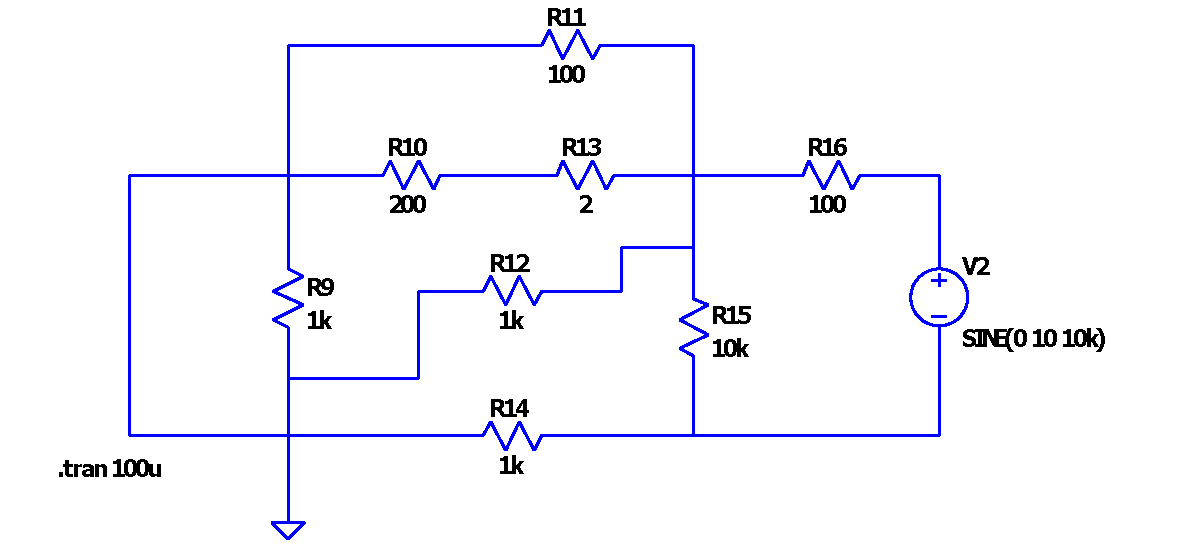
\includepdf[pages={1},scale=.8,pagecommand={}]{src/Schaltung4-1.pdf}
    \caption{LTSpice Simulation 1ste Tor}
    \label{fig:LTSpice1}
\end{figure}
\begin{figure}[H]
    \centering
    \includepdf[pages={2},scale=.8,pagecommand={}]{src/Schaltung4-1.pdf}
    \caption{LTSpice Simulation 2te Tor}
    \label{fig:LTspice2}
\end{figure}
%
Für die Simulation haben wir zwei Schaltungen gebaut, eine für das erste Tor und eine für das zweite Tor, mit der wir die folgenden Diagramme plotten können
%
\begin{flushright}
  \textit{\autorA}
\end{flushright}
%
%------------------------------%
%------ Ende eures Teils ------%
%------------------------------%
%
%
%